

%% AP Physics MC Questions Archive
%%----------------------------------------


%% Rotational Statics
%%----------------------------------------
\element{ap}{
\begin{question}{rotational-statics-q01}
    A bar of length $3d$ is pivoted in the center as shown.
    At each of its ends a force of magnitude $F$ is applied in the directions indicated by the arrows.
    \begin{center}
    \begin{tikzpicture}[font=\small,scale=1.1]
        %% Beam
        \draw[fill=white!90!black] (-3,0) rectangle (3,0.2);
        %% lengths
        \draw[<->] (-3,1) -- (-1.02,1) node[pos=0.5,anchor=center,fill=white] {$d$};
        \draw[<->] (-0.98,1) -- (-0.02,1) node[pos=0.5,anchor=center,fill=white] {$\dfrac{d}{2}$};
        \draw[<->] (0.02,1) -- (1,0.98) node[pos=0.5,anchor=center,fill=white] {$\dfrac{d}{2}$};
        \draw[<->] (1.02,1) -- (3,1) node[pos=0.5,anchor=center,fill=white] {$d$};
        %% point X
        \draw[fill] (-1,0.1) circle (1pt) node[anchor=north,yshift=-0.15] {$X$};
        %% Triangle
        \draw (0,0) -- ++(300:1) -- ++(180:1) -- cycle;
        %% Forces
        \draw[very thick,->] (-3,2) -- (-3,0.25);
        \draw[very thick,->] (+3,-1.95) -- (+3,-0.05);
    \end{tikzpicture}
    \end{center}
    What force must be applied at point $X$ to keep the rod in rotational equilibrium?
    \begin{multicols}{2}
    \begin{choices}
      \correctchoice{$6F$ upwards}
        \wrongchoice{$2F$ upwards}
        \wrongchoice{zero}
        \wrongchoice{$2F$ downwards}
        \wrongchoice{$6F$ downwards}
    \end{choices}
    \end{multicols}
\end{question}
}

\newcommand{\apRotationalStaticsQTwo}{
\begin{tikzpicture}
    %% Wall
    \draw (0,-1) -- (0,2);
    \node[anchor=west,fill,pattern=north east lines,minimum width=0.05cm, minimum height=3cm] at (0,0.5) {};
    %% Beam
    \draw[fill=white!50!black] (0,1ex) arc (90:270:1ex) --cycle;
    \draw[fill=white] (-0.9ex,1ex) rectangle (-4,-1ex);
    %% Vector
    \draw[very thick,->] (-3,1ex) -- (-3,2) node[anchor=west] {\SI{40}{\newton}};
\end{tikzpicture}
}

\element{ap}{
\begin{question}{rotational-statics-q02}
    %Base your answers to questions 2 and 3 on the picture below,
    The picture below represents a rigid uniform rod with a mass of \SI{6}{\kilo\gram} and a length of \SI{1.0}{\meter} is pivoted on the right end.
    It is held in equilibrium by an upward force of \SI{40}{\newton}.
    \begin{center}
        \apRotationalStaticsQTwo
    \end{center}
    How far from the left end of the rod should the force be placed to maintain equilibrium?
    \begin{multicols}{3}
    \begin{choices}
        \wrongchoice{\SI{10}{\centi\meter}}
        \wrongchoice{\SI{20}{\centi\meter}}
      \correctchoice{\SI{25}{\centi\meter}}
        \wrongchoice{\SI{40}{\centi\meter}}
        \wrongchoice{\SI{50}{\centi\meter}}
    \end{choices}
    \end{multicols}
\end{question}
}

\element{ap}{
\begin{question}{rotational-statics-q03}
    %Base your answers to questions 2 and 3 on the picture below,
    The picture below represents a rigid uniform rod with a mass of \SI{6}{\kilo\gram} and a length of \SI{1.0}{\meter} is pivoted on the right end.
    It is held in equilibrium by an upward force of \SI{40}{\newton}.
    \begin{center}
        \apRotationalStaticsQTwo
    \end{center}
    What force is applied to the rod by the pivot?
    \begin{multicols}{3}
    \begin{choices}
        \wrongchoice{\SI{10}{\newton}}
      \correctchoice{\SI{20}{\newton}}
        \wrongchoice{\SI{40}{\newton}}
        \wrongchoice{\SI{60}{\newton}}
        \wrongchoice{\SI{100}{\newton}}
    \end{choices}
    \end{multicols}
\end{question}
}

\element{ap}{
\begin{question}{rotational-statics-q04}
    The newton meter (\si{\newton\meter}) is a measure of:
    \begin{multicols}{2}
    \begin{choices}
        \wrongchoice{force}
      \correctchoice{torque}
        \wrongchoice{power}
        \wrongchoice{momentum}
        \wrongchoice{velocity}
    \end{choices}
    \end{multicols}
\end{question}
}

\newcommand{\apRotationalStaticsQFive}{
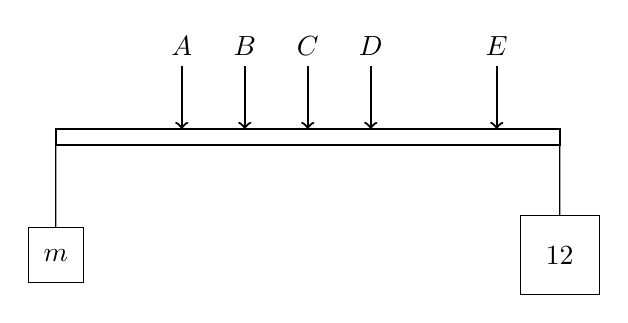
\begin{tikzpicture}[scale=0.8]
    %% NOTE:
    %% Bar, break into eighths
    \draw[thick] (-4,-0.25) rectangle (4,0);
    %\foreach \x in {-3,-2,..,2,3} {
    %    \draw (\x cm,-0.25) -- (\x cm,0);
    %}
    %% left weight
    \node[draw,minimum size=0.7cm] (L) at (-4,-2) {$m$};
    %% right weight
    \node[draw,minimum size=1cm] (R) at (4,-2) {\SI{12}{\kilo\gram}};
    %% Options, I,J,K,L,M
    \draw[thick,<-] (-2,0) -- (-2,1) node[anchor=south] {$A$};
    \draw[thick,<-] (-1,0) -- (-1,1) node[anchor=south] {$B$};
    \draw[thick,<-] (0,0) -- (0,1) node[anchor=south] {$C$};
    \draw[thick,<-] (1,0) -- (1,1) node[anchor=south] {$D$};
    \draw[thick,<-] (3,0) -- (3,1) node[anchor=south] {$E$};
    %% rope
    \draw (-4,0) -- (L.north);
    \draw (+4,0) -- (R.north);
\end{tikzpicture}
}

\element{ap}{
\begin{question}{rotational-statics-q05}
    Base your answers to questions 5 and 6 on the picture below,
        which represents two objects, one of mass \SI{12}{\kilo\gram} and one of mass $m$,
        hung from the ends of a stick with negligible mass,
        that is \SI{80}{\centi\meter} long and has marks every \SI{10}{\centi\meter} as shown below.
    \begin{center}
        \apRotationalStaticsQFive
    \end{center}
    If the stick remains horizontal when pivoted at point $B$,
        what is the mass of block $m$?
    \begin{multicols}{3}
    \begin{choices}
        \wrongchoice{\SI{7.2}{\kilo\gram}}
        \wrongchoice{\SI{7.5}{\kilo\gram}}
        \wrongchoice{\SI{12}{\kilo\gram}}
      \correctchoice{\SI{20}{\kilo\gram}}
        \wrongchoice{\SI{24}{\kilo\gram}}
    \end{choices}
    \end{multicols}
\end{question}
}

\element{ap}{
\begin{question}{rotational-statics-q06}
    Base your answers to questions 5 and 6 on the picture below,
        which represents two objects, one of mass \SI{12}{\kilo\gram} and one of mass $m$,
        hung from the ends of a stick with negligible mass,
        that is \SI{80}{\centi\meter} long and has marks every \SI{10}{\centi\meter} as shown below.
    \begin{center}
        \apRotationalStaticsQFive
    \end{center}
    If $m=\SI{7.2}{\kilo\gram}$,
        at what point should the rod be pivoted to remain horizontal?
    \begin{multicols}{3}
    \begin{choices}[o]
        \wrongchoice{$A$}
        \wrongchoice{$B$}
        \wrongchoice{$C$}
      \correctchoice{$D$}
        \wrongchoice{$E$}
    \end{choices}
    \end{multicols}
\end{question}
}

\element{ap}{
\begin{question}{rotational-statics-q07}
    Which of the following is not a scalar quantity?
    \begin{multicols}{2}
    \begin{choices}
        \wrongchoice{work}
        \wrongchoice{energy}
        \wrongchoice{speed}
      \correctchoice{torque}
        \wrongchoice{distance}
    \end{choices}
    \end{multicols}
\end{question}
}

\element{ap}{
\begin{question}{rotational-statics-q08}
    When an object is experiencing a net torque:
    \begin{choices}
        \wrongchoice{it is in dynamic equilibrium.}
        \wrongchoice{it is in static equilibrium.}
        \wrongchoice{it is rotating.}
      \correctchoice{it is translating.}
        \wrongchoice{its mechanical energy is negative.}
    \end{choices}
\end{question}
}

\element{ap}{
\begin{question}{rotational-statics-q09}
    A uniform wooden board of mass $10 M$ is held up by a nail hammered into a wall.
    A block of mass $M$ rests $L/2$ away from the pivot.
    Another block of a certain mass is hung a distance $L/3$.
    The system is in static equilibrium.
    \begin{center}
    \begin{tikzpicture}
        %% TODO: draw tikz
    \end{tikzpicture}
    \end{center}
    %% NOTE: change ? to X
    What is the measure of the mass labeled ``?''?
    \begin{multicols}{3}
    \begin{choices}
        \wrongchoice{$\dfrac{M}{2}$}
        \wrongchoice{$\dfrac{M}{3}$}
        \wrongchoice{$M$}
      \correctchoice{$\dfrac{3M}{2}$}
        \wrongchoice{$2M$}
    \end{choices}
    \end{multicols}
\end{question}
}

\newcommand{\apRotationalStaticsQTen}{
\begin{tikzpicture}
    %% TODO: draw tikz
    %% Rigid rod
    \draw(0,0) rectangle (6,0.1);
    \foreach \i in {1,2,3,4,5}
        \draw (\i,0.1) -- (\i,0.0);
    %% Forces
    \draw (1,0) -- ++(215:2) node[anchor=north] {$F$};
    \draw (1,0) ++(180:1) arc(180:215:1) node[pos=0.5,anchor=east] {\ang{45}};
    \draw (3,0.1) -- ++(90:2) node[pos=0.5,anchor=west] {$5F$};
    \draw (6,0.1) -- ++(45:2) node[pos=0.5,anchor=west] {$2F$};
    \draw (6,0.1) -- ++(0:1.5);
    \draw (6,0.1) ++(0:1) arc(0:45:1) node[pos=0.5,anchor=west] {\ang{45}};
    \draw (6,0) -- ++(90:2) node[anchor=west] {$\dfrac{F}{2}$};
\end{tikzpicture}
}

\element{ap}{
\begin{question}{rotational-statics-q10}
    %% Base your answers to questions 10 and 11 on the following information.
    A uniform rod of length $L$ is placed into outer space with the following forces acting on it:
    \begin{itemize}
        \itemsep=0pt
        \item $5F$ upwards from its center of mass.
        \item $F$ at \ang{45} downwards $\dfrac{L}{3}$ from its center of mass.
        \item $2F$ at \ang{45} upwards $\dfrac{L}{2}$ from its center of mass.
        \item $\dfrac{F}{2}$ downwards $\dfrac{L}{2}$ from its center of mass.
    \end{itemize}
    \begin{center}
        \apRotationalStaticsQTen
    \end{center}
    If this object is to rotate,
        which way would it be?
    \begin{choices}
        \wrongchoice{It will rotate Clockwise.}
      \correctchoice{It will rotate Counter-Clockwise.}
        \wrongchoice{It will rotate in dynamic equilibrium.}
        \wrongchoice{It will not rotate, it will only move upwards.}
        \wrongchoice{It will not rotate it will only move downwards.}
    \end{choices}
\end{question}
}

\element{ap}{
\begin{question}{rotational-statics-q11}
    %% Base your answers to questions 10 and 11 on the following information.
    A uniform rod of length $L$ is placed into outer space with the following forces acting on it:
    \begin{itemize}
        \item $5F$ upwards from its center of mass.
        \item $F$ at \ang{45} downwards $\dfrac{L}{3}$ from its center of mass.
        \item $2F$ at \ang{45} upwards $\dfrac{L}{2}$ from its center of mass.
        \item $\dfrac{F}{2}$ downwards $\dfrac{L}{2}$ from its center of mass.
    \end{itemize}
    \begin{center}
        \apRotationalStaticsQTen
    \end{center}
    What is the magnitude of the force needed to bring this object into translational equilibrium?
    \begin{choices}
        %% TODO: question formating
      \correctchoice{$X: F 2 `2 2 Y: F(9 + `2)$}
        \wrongchoice{$X: F 2 Y: F(9 – `2)$}
        \wrongchoice{$X: ( F 2 ) 2 Y: 7F$}
        \wrongchoice{$X: F(9 – `2) Y: F 2 `2 2$}
        \wrongchoice{$X: F(9 – `2) Y: F 2 `2 2$}
    \end{choices}
\end{question}
}

\element{ap}{
\begin{question}{rotational-statics-q12}
    A person of mass \SI{60}{\kilo\gram} is walking down a \SI{10}{\meter},
        \SI{100}{\kilo\gram} beam supported by two pillars,
        one at the head of the beam and one \SI{3}{\meter} away from the center of the beam.
    \begin{center}
    \begin{tikzpicture}
        %% TODO: draw tikz
    \end{tikzpicture}
    \end{center}
    How far down the beam can the person walk before the beam begins to tip?
    (Consider the origin to be the left end of the beam.)
    \begin{multicols}{2}
    \begin{choices}
        \wrongchoice{\SI{0}{\meter}}
        \wrongchoice{\SI{2}{\meter}}
      \correctchoice{\SI{7/3}{\meter}}
        \wrongchoice{\SI{20/3}{\meter}}
        \wrongchoice{To the end of the beam}
    \end{choices}
    \end{multicols}
\end{question}
}

\element{ap}{
\begin{question}{rotational-statics-q13}
    In the diagram below a mass $m$ is attached by a massless string to a stationary arm at an angle $\theta$ from the horizontal.
    \begin{center}
    \begin{tikzpicture}
        %% ceiling
        \draw (-1,0) -- (3,0);
        \node[anchor=south,fill,pattern=north east lines,minimum width=4cm, minimum height=0.1cm] at (1,0) {};
        %% hinge and rod
        \draw[fill=white!90!black] (-0.2,0) arc(180:356:0.2) --cycle;
        \draw[fill=white]          (-0.1,0) arc(180:360:0.1) --cycle;
        \draw[fill=white!90!black,rotate around={45:(0,0)}] (-0.2,-0.2) rectangle (0.2,-4);
        %% angle
        \draw[<->] (2.25,0) arc (0:-45:2) node[pos=0.5,anchor=center,fill=white] {\ang{60}};
        %% mass
        \node[draw,circle,minimum size=1cm,fill=white!90!black,anchor=north] (M) at (2.75,-4) {$m$};
        \draw[thick]  (M.north) -- (2.83,-2.83);
    \end{tikzpicture}
    \end{center}
    If the net torque of the mass on the arm is $\tau$,
        find the length of the lever arm.
    \begin{multicols}{2}
    \begin{choices}
        \wrongchoice{$\dfrac{\tau}{mg\sin\theta}$}
      \correctchoice{$\dfrac{\tau}{mg\cos\theta}$}
        \wrongchoice{$\dfrac{mg\cos\theta}{\tau}$}
        \wrongchoice{$\dfrac{mg\sin\theta}{\tau}$}
        \wrongchoice{$\dfrac{\tau}{mg\sin\theta\cos\theta}$}
    \end{choices}
    \end{multicols}
\end{question}
}

\element{ap}{
\begin{question}{rotational-statics-q14}
    In the diagram above, two masses, one with mass $m$,
        the other with mass $M=2m$ are resting on a uniform plank of length $L$ that pivots at its midpoint.
    \begin{center}
    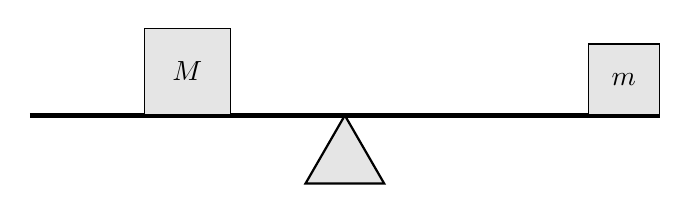
\begin{tikzpicture}
        %% beam
        \draw[ultra thick] (-4,0) -- (4,0);
        %% triangle
        \draw[thick,fill=white!90!black] (0,0) -- ++(300:1) --++(180:1) -- cycle;
        %% masses
        \node[draw,fill=white!90!black,minimum size=0.9cm,anchor=south east] at (4,0) {$m$};
        \node[draw,fill=white!90!black,minimum size=1.1cm,anchor=south] at (-2,0) {$M$};
    \end{tikzpicture}
    \end{center}
    If the mass $m$ is at the far end of the plank,
        how far away from the pivot should the mass $M$ be to balance the plank in a horizontal position shown?
    \begin{multicols}{3}
    \begin{choices}
        \wrongchoice{$\dfrac{L}{2}$}
        \wrongchoice{$\dfrac{L}{3}$}
      \correctchoice{$\dfrac{L}{4}$}
        \wrongchoice{$\dfrac{L}{6}$}
        \wrongchoice{$2L$}
    \end{choices}
    \end{multicols}
\end{question}
}

\element{ap}{
\begin{question}{rotational-statics-q15}
    The diagram above shows a massless pole of length $L$ that supports a mass $m$ being held horizontally against a tower by a wire that makes an angle $\theta$ with the horizontal pole.
    The wire is connected to the pole at a distance $x$ from the free end of the pole.
    The mass is attached by a massless string at the free end of the pole.
    \begin{center}
    \begin{tikzpicture}
        %% Wall
        \draw (0,-2) -- (0,4);
        \node[anchor=east,fill,pattern=north east lines,minimum width=0.05cm, minimum height=6cm] at (0,1) {};
        %% hinge and rod
        \draw[fill=white!90!black] (0,-0.1) arc(-90:90:0.1) --cycle;
        \draw[fill=white!90!black] (+0.1,-0.1) rectangle (6,0.1);
        %\draw (0.2,0.1) -- (0.2,0.3) -- (0,0.3); 
        %% rope and angle
        \draw[very thick] (5,0.1) -- (0,3.1);
        \draw[<->] (4,0.1) arc(180:149:1) node[pos=0.5,anchor=east] {$\theta$};
        %% mass
        \node[draw,fill=white!90!black,minimum size=1cm,anchor=north] (M) at (6,-1.5) {$m$};
        \draw[very thick] (M.north) -- (6,0.1);
        %% distances
        \draw[<->] (6,1) -- (5,1) node[pos=0.5,anchor=south] {$x$};
        \draw[<->] (5,-1) -- (0,-1) node[pos=0.5,anchor=center,fill=white] {$L-x$};
    \end{tikzpicture}
    \end{center}
    For the pole to remain horizontal,
        the tension in the wire must be:
    \begin{multicols}{2}
    \begin{choices}
        \wrongchoice{$\dfrac{mgL}{2x\cos\theta}$}
        \wrongchoice{$\dfrac{mgx}{2L\cos\theta}$}
        \wrongchoice{$\dfrac{mgx}{2(L-x)\sin\theta}$}
      \correctchoice{$\dfrac{mgL}{(1-x)\sin\theta}$}
        \wrongchoice{$\dfrac{mgL}{2(L-x)\sin\theta}$}
    \end{choices}
    \end{multicols}
\end{question}
}

\element{ap}{
\begin{question}{rotational-statics-q16}
    The diagram above shows a stick of uniform density with length $2L$ and mass $m$ supported near each end by upward forces.
    \begin{center}
    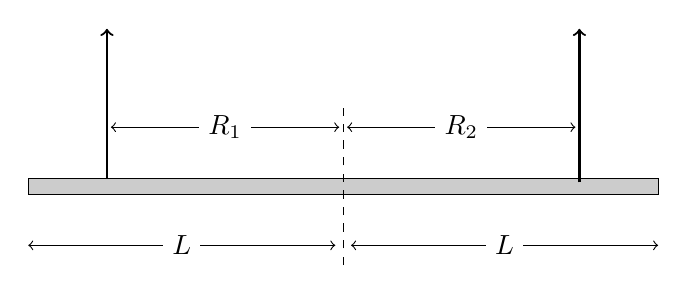
\begin{tikzpicture}
        %% Stick
        \draw[fill=white!80!black] (-4,-0.1) rectangle (4,0.1);
        %% Length L
        \draw[<->] (-4,-0.75) -- (-0.1,-0.75) node[pos=0.5,anchor=center,fill=white] {$L$};
        \draw[<->] (+4,-0.75) -- (+0.1,-0.75) node[pos=0.5,anchor=center,fill=white] {$L$};
        %% R_1 and R_2
        \draw[dashed] (0,-1) -- (0,1);
        \draw[thick,->] (-3,0.1) -- (-3,2);
        \draw[<->] (-2.95,0.75) -- (-0.05,0.75) node[pos=0.5,anchor=center,fill=white] {$R_1$};
        \draw[thick,->] (+3,0.05) -- (+3,2);
        \draw[<->] (+2.95,0.75) -- (+0.05,0.75) node[pos=0.5,anchor=center,fill=white] {$R_2$};
    \end{tikzpicture}
    \end{center}
    Find the magnitude of the force a distance $R_1$ away from the center of the stick if the stick is balanced in a horizontal position.
    \begin{multicols}{2}
    \begin{choices}
        \wrongchoice{$\dfrac{mgR_2}{R_1}$}
        \wrongchoice{$\dfrac{mgR_1}{R_2}$}
        \wrongchoice{$\dfrac{mg\left(R_1+R_2\right)}{R_1}$}
      \correctchoice{$\dfrac{mgR_2}{R_1+R_2}$}
        \wrongchoice{$\dfrac{mgR_1}{R_1+R_2}$}
    \end{choices}
    \end{multicols}
\end{question}
}

\element{ap}{
\begin{question}{rotational-statics-q17}
    If the rod in the figure above is uniform with mass $m$,
    \begin{center}
    \begin{tikzpicture}
        %% Wall
        \draw (0,-1) -- (0,4);
        \node[anchor=east,fill,pattern=north east lines,minimum width=0.05cm, minimum height=5cm] at (0,1.5) {};
        %\draw (0.2,0.1) -- (0.2,0.3) -- (0,0.3); 
        %% hinge and rod
        \draw[fill=white!90!black] (0,-0.1) arc(-90:90:0.1) --cycle;
        \draw[fill=white!90!black] (+0.1,-0.1) rectangle (5,0.1);
        \node[anchor=south] at (2,0.1) {rod};
        %% rope and angle
        \draw[very thick] (5,0.1) -- (0,3.1) node[pos=0.5,anchor=south,rotate=-30] {string};
        \draw[<->] (3.5,0.1) arc(180:149:1.5) node[pos=0.5,anchor=east] {$\theta$};
    \end{tikzpicture}
    \end{center}
        what is the tension in the supporting string?
    \begin{multicols}{2}
    \begin{choices}
        \wrongchoice{$mg\sin\theta$}
        \wrongchoice{$\dfrac{mg\sin\theta}{2}$}
        \wrongchoice{$\dfrac{mg\cos\theta}{2}$}
        \wrongchoice{$\dfrac{mg}{2\cos\theta}$}
      \correctchoice{$\dfrac{mg}{2\sin\theta}$}
    \end{choices}
    \end{multicols}
\end{question}
}

\element{ap}{
\begin{question}{rotational-statics-q18}
    The rod in the figure below is uniform,
        and the tension in the string is $T$.
    \begin{center}
    \begin{tikzpicture}
        %% NOTE:
    \end{tikzpicture}
    \end{center}
    The mass of the rod is:
    \begin{multicols}{3}
    \begin{choices}
        \wrongchoice{$2Tg$}
      \correctchoice{$\dfrac{2T}{g}$}
        \wrongchoice{$\dfrac{T}{g}$}
        \wrongchoice{$\dfrac{T}{2g}$}
        \wrongchoice{$\dfrac{2g}{T}$}
    \end{choices}
    \end{multicols}
\end{question}
}

\element{ap}{
\begin{question}{rotational-statics-q19}
    To measure the weight of the cat,
        a person places a \SI{100}{\newton} box and a \SI{60}{\newton} box from the ends of a uniform pole that is pivoted at its center.
    \begin{center}
    \begin{tikzpicture}
        %% NOTE:
    \end{tikzpicture}
    \end{center}
    The system balances when the cat stands at a point $\dfrac{1}{4}$ of the rods length from the \SI{60}{\newton} box.
    What is the approximate mass of the cat?
    \begin{multicols}{3}
    \begin{choices}
        \wrongchoice{\SI{3}{\kilo\gram}}
        \wrongchoice{\SI{4}{\kilo\gram}}
        \wrongchoice{\SI{6}{\kilo\gram}}
      \correctchoice{\SI{8}{\kilo\gram}}
        \wrongchoice{\SI{12}{\kilo\gram}}
    \end{choices}
    \end{multicols}
\end{question}
}

\element{ap}{
\begin{question}{rotational-statics-q20}
    A rod of uniform material is balanced over a pivot with masses $m$ and $M$ positioned such that the system is in static equilibrium.
    If the mass $M$ is a distance $d$ from the pivot,
        and the mass $m$ is a distance $\dfrac{d}{4}$ from the pivot,
        what is the ratio of $M$ to $m$?
    \begin{multicols}{3}
    \begin{choices}
        \wrongchoice{$4:1$}
        \wrongchoice{$2:1$}
        \wrongchoice{$1:1$}
        \wrongchoice{$1:2$}
      \correctchoice{$1:4$}
    \end{choices}
    \end{multicols}
\end{question}
}

\element{ap}{
\begin{question}{rotational-statics-q21}
    A massless rod is positioned on a frictionless pivot as shown.
    A force with magnitude $F$ is applied at an angle $\theta$,
        a distance $L$ from the pivot.
    \begin{center}
    \begin{tikzpicture}
        %% NOTE:
    \end{tikzpicture}
    \end{center}
    At what distance $x$ must the same force $F$ be applied perpendicular to the rod such that the net torque on the rod is zero?
    \begin{multicols}{3}
    \begin{choices}
      \correctchoice{$L\sin\theta$}
        \wrongchoice{$L\cos\theta$}
        \wrongchoice{$L$}
        \wrongchoice{$L\tan\theta$}
        \wrongchoice{$\sqrt{2}L$}
    \end{choices}
    \end{multicols}
\end{question}
}

\element{ap}{
\begin{question}{rotational-statics-q22}
    %% Base your answer to the following question on
    The diagram below shows a uniform disc connected to a massless string of tension $T$.
    \begin{center}
    \begin{tikzpicture}
        %% NOTE:
    \end{tikzpicture}
    \end{center}
    %% Add I is the momentu of intertia and r is the radius of the disc
    What is $T$ if the object is initially at rest?
    \begin{multicols}{3}
    \begin{choices}
      \correctchoice{zero}
        \wrongchoice{$\dfrac{Ig}{2r^2}$}
        \wrongchoice{$\dfrac{Ig}{r^2}$}
        \wrongchoice{$\dfrac{2Ig}{r^2}$}
        \wrongchoice{$\dfrac{2Ig}{r}$}
    \end{choices}
    \end{multicols}
\end{question}
}


\endinput


